\PassOptionsToPackage{unicode=true}{hyperref} % options for packages loaded elsewhere
\PassOptionsToPackage{hyphens}{url}
\documentclass[12pt,ignorenonframetext,aspectratio=169]{beamer}
\IfFileExists{pgfpages.sty}{\usepackage{pgfpages}}{}
\setbeamertemplate{caption}[numbered]
\setbeamertemplate{caption label separator}{: }
\setbeamercolor{caption name}{fg=normal text.fg}
\beamertemplatenavigationsymbolsempty
\usepackage{lmodern}
\usepackage{amssymb}
\usepackage{amsmath}
\usepackage{ifxetex,ifluatex}
\usepackage{fixltx2e} % provides \textsubscript
\ifnum 0\ifxetex 1\fi\ifluatex 1\fi=0 % if pdftex
  \usepackage[T1]{fontenc}
  \usepackage[utf8]{inputenc}
\else % if luatex or xelatex
  \ifxetex
    \usepackage{mathspec}
  \else
    \usepackage{fontspec}
\fi
\defaultfontfeatures{Ligatures=TeX,Scale=MatchLowercase}






%
\fi

  \usetheme[]{iqss}






% use upquote if available, for straight quotes in verbatim environments
\IfFileExists{upquote.sty}{\usepackage{upquote}}{}
% use microtype if available
\IfFileExists{microtype.sty}{%
  \usepackage{microtype}
  \UseMicrotypeSet[protrusion]{basicmath} % disable protrusion for tt fonts
}{}


\newif\ifbibliography


\hypersetup{
      pdftitle={National and international trade of in High Value Crops (HVCs)},
        pdfauthor={Deependra Dhakal},
          pdfborder={0 0 0},
    breaklinks=true}
%\urlstyle{same}  % Use monospace font for urls







% Prevent slide breaks in the middle of a paragraph:
\widowpenalties 1 10000
\raggedbottom

  \AtBeginPart{
    \let\insertpartnumber\relax
    \let\partname\relax
    \frame{\partpage}
  }
  \AtBeginSection{
    \ifbibliography
    \else
      \let\insertsectionnumber\relax
      \let\sectionname\relax
      \frame{\sectionpage}
    \fi
  }
  \AtBeginSubsection{
    \let\insertsubsectionnumber\relax
    \let\subsectionname\relax
    \frame{\subsectionpage}
  }



\setlength{\parindent}{0pt}
\setlength{\parskip}{6pt plus 2pt minus 1pt}
\setlength{\emergencystretch}{3em}  % prevent overfull lines
\providecommand{\tightlist}{%
  \setlength{\itemsep}{0pt}\setlength{\parskip}{0pt}}

  \setcounter{secnumdepth}{0}


  \usepackage{booktabs}
  \usepackage{longtable}
  \usepackage{emptypage}
  \usepackage{array}
  \usepackage{multirow}
  \usepackage{wrapfig}
  \usepackage{float}
  \usepackage{colortbl}
  \usepackage{pdflscape}
  \usepackage{tabu}
  \usepackage{threeparttable}
  \usepackage{threeparttablex}
  \usepackage[normalem]{ulem}
  \usepackage{rotating}
  \usepackage{makecell}
  \usepackage{xcolor}
  \usepackage{tikz} % required for image opacity change
  \usepackage[absolute,overlay]{textpos} % for text formatting
  \usepackage[utf8]{inputenc}
  \usetikzlibrary{mindmap,arrows,shapes,positioning,shadows,trees}
  \usepackage[skip=2pt]{caption}

  % this font option is amenable for beamer
  \setbeamerfont{caption}{size=\tiny}


%% IQSS overrides
\iqsssectiontitle{Outline}

\AtBeginSection[]{
  \title{\insertsectionhead}
  {
    \definecolor{white}{rgb}{0.776,0.357,0.157}
    \definecolor{iqss@orange}{rgb}{1,1,1}
    \ifnum \insertmainframenumber > \insertframenumber
    \frame{
      \frametitle{\iqsssectiontitleheader}
      \tableofcontents[currentsection]
    }
    \else
    \frame{
      \frametitle{Backup Slides}
      \tableofcontents[sectionstyle=shaded/shaded,subsectionstyle=shaded/shaded/shaded]
    }
    \fi
  }
}

\AtBeginSubsection[]{}

%%


  \title[]{National and international trade of in High Value Crops
(HVCs)}



  \author[
        Deependra Dhakal
    ]{Deependra Dhakal}

  \institute[
    ]{
    GAASC, Baitadi \and Tribhuwan University
    }

\date[
      \today
  ]{
      \today
        }

\begin{document}

% Hide progress bar and footline on titlepage
  \begin{frame}[plain]
  \titlepage
  \end{frame}



\hypertarget{trade}{%
\section{Trade}\label{trade}}

\begin{frame}{Background}
\protect\hypertarget{background}{}
\begin{itemize}
\tightlist
\item
  Involves the buying and selling of goods and services
\item
  International trade allows countries expand their markets for goods
  and services that otherwise may not have been available
\item
  International trade makes the trade more competitive and brings
  cheaper goods home.
\end{itemize}
\end{frame}

\begin{frame}{}
\protect\hypertarget{section}{}
\textbf{Export}

\begin{itemize}
\tightlist
\item
  Export to send good to another country for sale. -- Advance Learner
  Dictionary
\item
  To send goods or services across national frontiers for the purpose of
  selling and realizing foreign exchange.
\end{itemize}

\textbf{Import}

\begin{itemize}
\tightlist
\item
  Import; to buy or bring in products from another country. -- Advance
  Learner Dictionary
\item
  ``Imports'' consist of transactions in goods and services (sales,
  barter, gifts or grants) from non-resident residents to residents.
\item
  An import of a good occurs when there is a change of ownership from a
  non-resident to a resident;
\item
  This does not necessarily imply that the good in question physically
  crosses the frontier. Also smuggled goods be included in the import
  measurement.
\end{itemize}
\end{frame}

\hypertarget{policies-and-agreements-in-trade}{%
\section{Policies and agreements in
trade}\label{policies-and-agreements-in-trade}}

\begin{frame}{National policies}
\protect\hypertarget{national-policies}{}
\begin{itemize}
\tightlist
\item
  Fiscal policy
\item
  Trade strategies (NTIS)
\item
  National trade policy (1992, 2015)

  \begin{itemize}
  \tightlist
  \item
    First trade policy introduced in 1983 with the slogan of ``Exports
    for development''
  \item
    Trade policy, 1992 removed most of the trade barriers such as
    eliminating licensing for import and export, establishing industry,
    etc.
  \item
    Trade policy, 2015 highlights:

    \begin{itemize}
    \tightlist
    \item
      Trade in goods, trade in services and trade in intellectural
      property rights
    \item
      Trade related infrastructure building
    \item
      Product development and value chains
    \item
      Capacity development and export promotion
    \item
      Trade facilitation
    \item
      Participation in the global production chains and value chains
    \item
      Market access/promotion/diversification
    \item
      Resource mobilization (Aid for trade), Trade related technical
      assistance
    \end{itemize}
  \end{itemize}
\end{itemize}
\end{frame}

\begin{frame}{International treaties and agreements}
\protect\hypertarget{international-treaties-and-agreements}{}
\begin{enumerate}
\tightlist
\item
  Indo-Nepal trade treaty
\item
  China-Nepal trade treaty
\item
  South Asian Free Trade Area (SAFTA): It provides the basis for trade
  liberalization programmes for LDCs and non-LDCs separately, in terms
  of tariff reductions and inclusion of products in the sensitive list.
  (Bangladesh, Bhutan, Maldives, Nepal, India, Pakistan, and Sri Lanka,
  Afghanistan)
\item
  Bay of Bengal Initiative for Multi-Sectoral Technical and Economic
  Cooperation (BIMISTEC): The aim of the Framework Agreement is to
  stimulate trade and investment among the parties, and to attract trade
  and investment from outside. (India, Sri Lanka, and Thailand,
  Bangladesh, Bhutan, Myanmar, and Nepal)
\item
  World Trade Organization (WTO): Nepal has been a WTO Member since 23
  April 2004 when it became the first least developed country (LDC) to
  join the WTO through the full working party negotiation process.
\end{enumerate}

\begin{itemize}
\tightlist
\item
  AOA, TRIPS, SPS
\item
  International agreements
\end{itemize}
\end{frame}

\hypertarget{implications-of-national-trade-of-hvcs}{%
\section{Implications of national trade of
HVCs}\label{implications-of-national-trade-of-hvcs}}

\begin{frame}{High value crops}
\protect\hypertarget{high-value-crops}{}
\begin{table}

\caption{\label{tab:high-value-crops}Traditional and high value agricultural commodities}
\centering
\fontsize{8}{10}\selectfont
\begin{tabular}[t]{ll}
\toprule
Traditional & Non-traditional (HVA)\\
\midrule
Sugar & Dairy products\\
Cotton & Meat products\\
Jute & Vegetables\\
Tobacco & Fruit\\
Coffee & Fish\\
\addlinespace
Cocoa & NTF products, nuts\\
Tea & Species and essential oils\\
Bananas & Herbs\\
Cereals, roots and tubers & \\
Oilseeds & \\
\bottomrule
\end{tabular}
\end{table}
\end{frame}

\begin{frame}{Implications of national trade}
\protect\hypertarget{implications-of-national-trade}{}
\begin{itemize}
\tightlist
\item
  Access to cheaper and nutritious food source to citizens of all
  geographical regions
\item
  Strengthening of development infrastructures -- transport,
  electricity, communication channels
\item
  More balanced economic and physical growth
\item
  Affordable access to HVCs will direct competitive production of other
  agricultural commodities
\item
  Equitable share of food items helps in achieving food security
\item
  Opportunity for quality awareness in local consumers
\item
  Establishment of small and medium scale processing agribusiness
  enterprises.
\end{itemize}
\end{frame}

\hypertarget{implications-of-international-trade-in-agriculture-sector}{%
\section{Implications of international trade in agriculture
sector}\label{implications-of-international-trade-in-agriculture-sector}}

\begin{frame}{}
\protect\hypertarget{section-1}{}
\begin{itemize}
\tightlist
\item
  Nepal is a net importer of agricultural products
\item
  Exports of agricultural products declined in 2015 compared to 2013 and
  2014
\item
  Nepalese economy is still dependent highly on tariff revenue
\item
  Nepal imports pretty much all types of goods and services that are
  consumed in the domestic market
\item
  Causes of import:

  \begin{itemize}
  \tightlist
  \item
    Import share of petroleum products is about 25\%.
  \item
    The process of development caused increased import
  \item
    Increase in purchasing power of the people
  \item
    Weak commercialization and negotiation ability
  \item
    Standard issues
  \end{itemize}
\end{itemize}
\end{frame}

\begin{frame}{}
\protect\hypertarget{section-2}{}
\begin{figure}
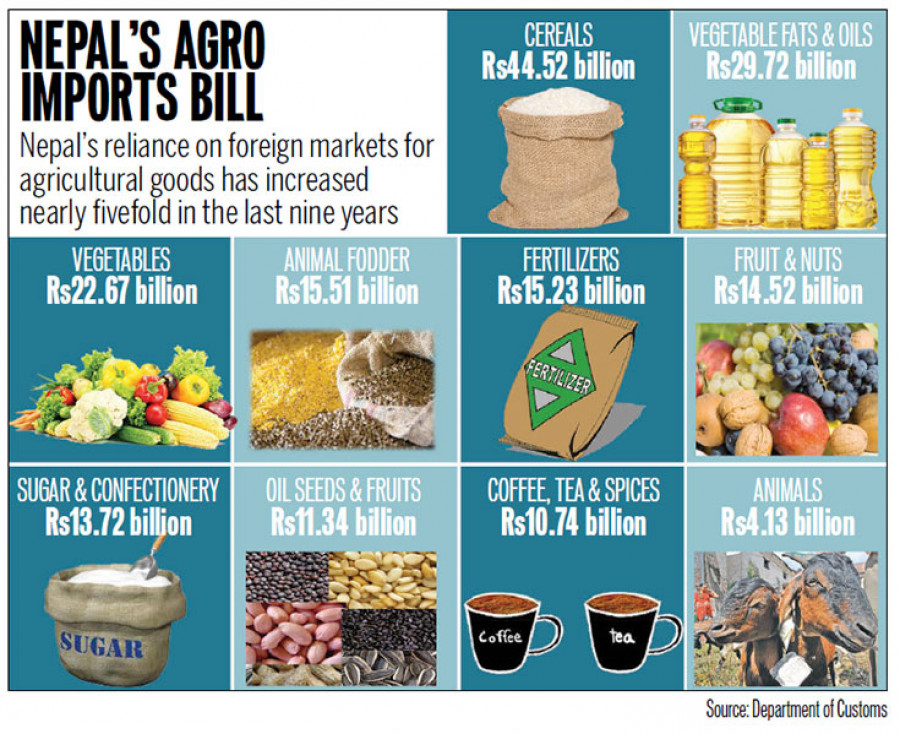
\includegraphics[width=0.8\linewidth]{./figs/nepal_agri_import_bill_2018} \caption{Food import expenses for Nepal during year 2018 AD}\label{fig:food-import-nepal}
\end{figure}
\end{frame}

\begin{frame}{Impacts of trade liberalization and WTO in agriculture}
\protect\hypertarget{impacts-of-trade-liberalization-and-wto-in-agriculture}{}
\begin{itemize}
\tightlist
\item
  Opportunities:

  \begin{enumerate}
  \tightlist
  \item
    Market access
  \item
    Attract foreign direct investment
  \item
    Improvement of domestic institutional capability
  \item
    Benefit from liberalization
  \item
    Access to dispute settlement body
  \item
    Mobilization of trade related technical assistance
  \end{enumerate}
\end{itemize}
\end{frame}

\begin{frame}{}
\protect\hypertarget{section-3}{}
\begin{itemize}
\tightlist
\item
  Challenges:

  \begin{itemize}
  \tightlist
  \item
    Nepal's widening trade deficit due to increasing import as result of
    easy access of foreign products in our market
  \item
    Lack of trading infrastructure making Nepalese products difficult to
    compete in world market
  \item
    Limited availability of Sanitary and Phytosanitary quarantine
    inspection and food testing lab at border in Nepal
  \item
    Reduction in export subsidy that demotivated the exporting producers
  \item
    Lack of quality and quantity production of agriculture products
    which made it less competitive in world market
  \end{itemize}
\end{itemize}
\end{frame}




\end{document}
